\chapter{Correlation}

This chapter provides a graphical representation of how correlation is
performed in Ames Stereo Pipeline. Most importantly this provides a
quick comparison of different algorithms provided to save the user the
time of comparing results themselves.

For this chapter we'll be using the north most tip of Hadley Rille as
captured by the Apollo 15 Metric Camera. Here's what the left and right
pair looks like before any processing has been applied. The right image
is actually larger than the left.

\begin{figure}[hb]
\centering
  \subfigure[{\tt Left}]{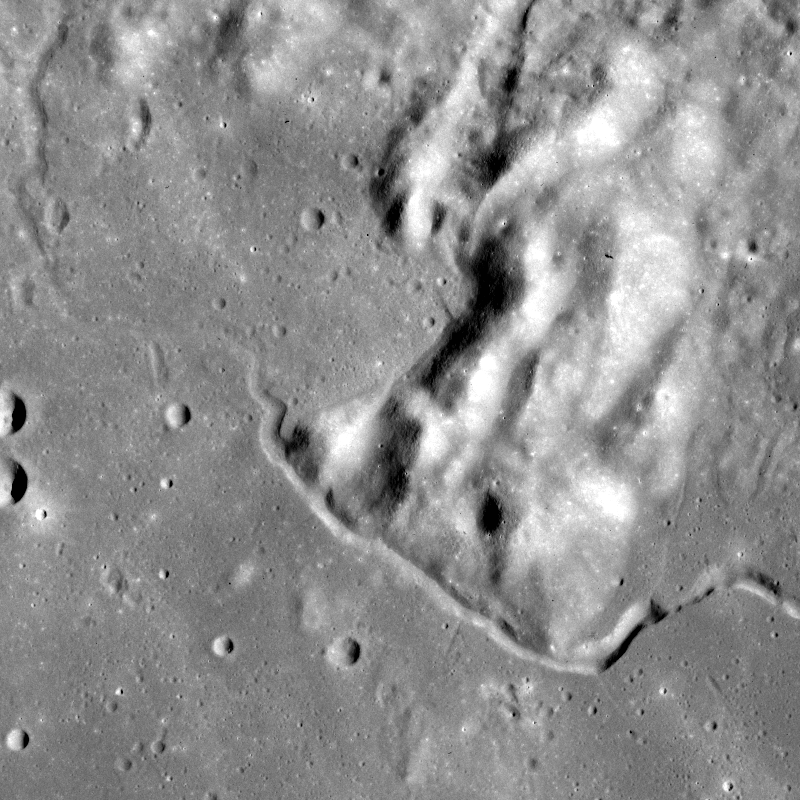
\includegraphics[width=3in]{images/correlation/sub4-AS15-M-1134_crop.png}\label{fig:left_input_image}}
  \hfil
  \subfigure[{\tt Right}]{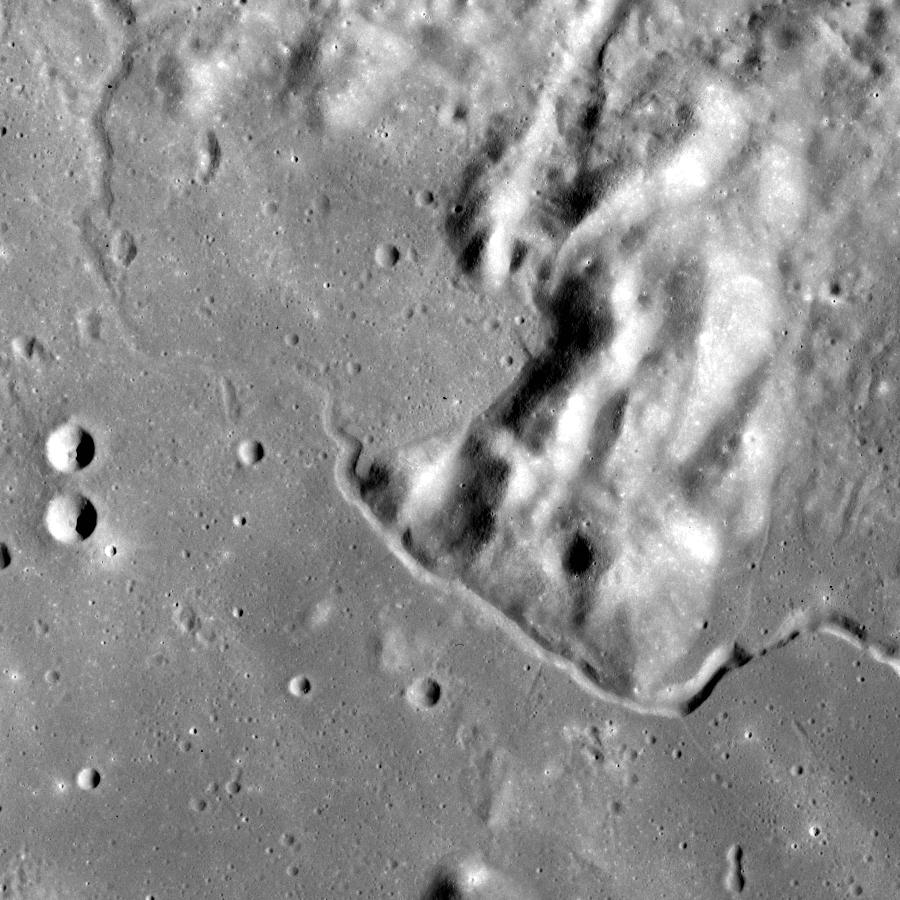
\includegraphics[width=3in]{images/correlation/sub4-AS15-M-1135_crop.png}\label{fig:right_input_image}}
\caption{Original input images used for this chapter.}
\label{fig:input_images}
\end{figure}

\section{Preprocessing Filters and Integer Correlation}

\subsection{Cost Functions}

\subsection{Gaussian Blur}

\subsection{Log Filter}

\subsection{SLog Filter}

\subsection{Pyramid Correlator}

\section{Sub-pixel Correlation}

\subsection{Parabola}

\begin{figure}[hb]
\centering
  \subfigure[{\tt 3D result}]{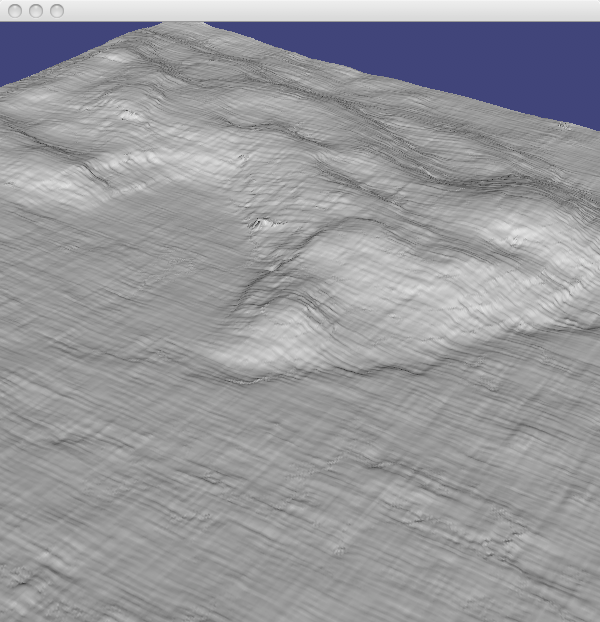
\includegraphics[width=3in]{images/correlation/3D_mode0.png}}
  \hfil
  \subfigure[{\tt Hillshade Result}]{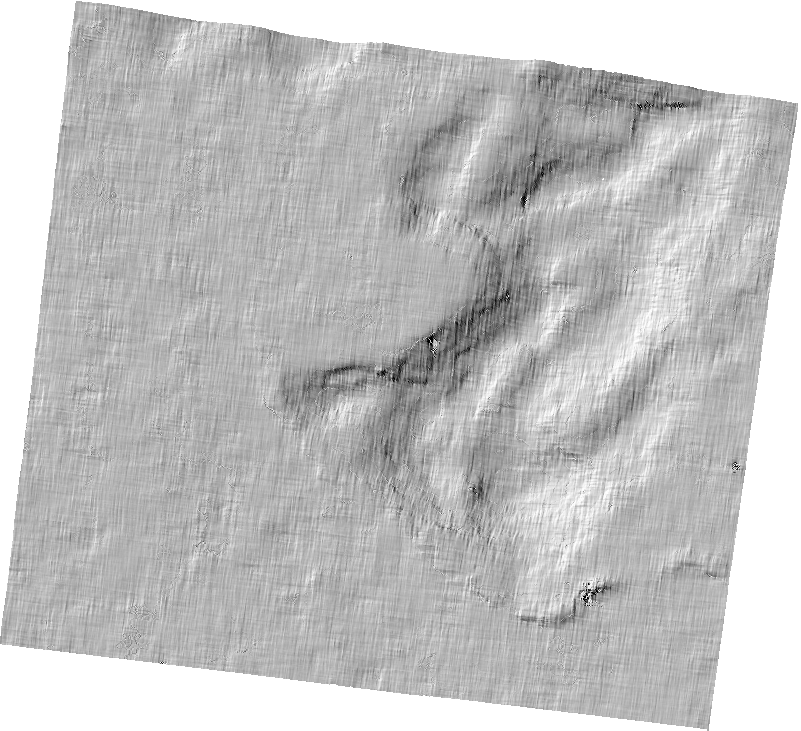
\includegraphics[width=3in]{images/correlation/hillshade_mode0.png}}
\caption{Results using Parabola subpixel mode.}
\label{fig:parabola_results}
\end{figure}

\subsection{Robust weighted Affine}

\begin{figure}[hb]
\centering
  \subfigure[{\tt 3D result}]{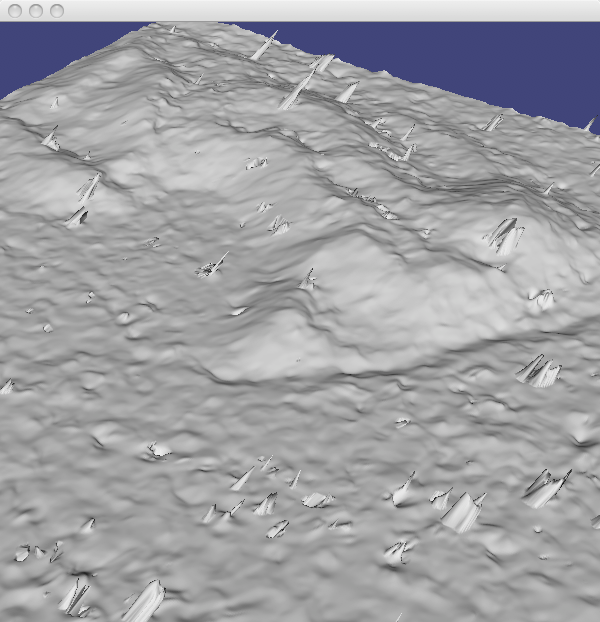
\includegraphics[width=3in]{images/correlation/3D_mode1.png}}
  \hfil
  \subfigure[{\tt Hillshade Result}]{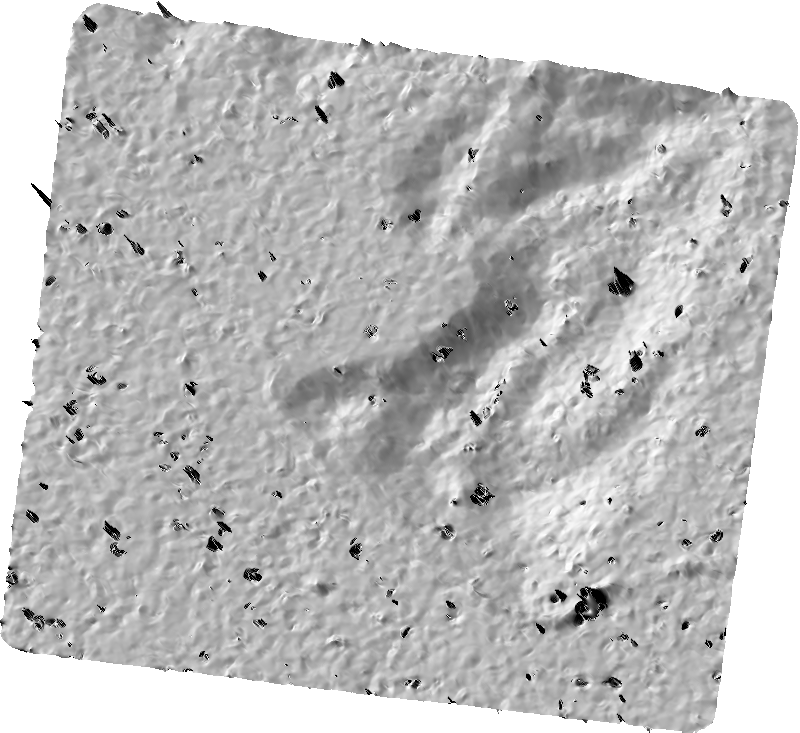
\includegraphics[width=3in]{images/correlation/hillshade_mode1.png}}
\caption{Results using Robust Affine subpixel mode.}
\label{fig:robust_results}
\end{figure}

\subsection{Bayes weighted Affine}

\begin{figure}[hb]
\centering
  \subfigure[{\tt 3D result}]{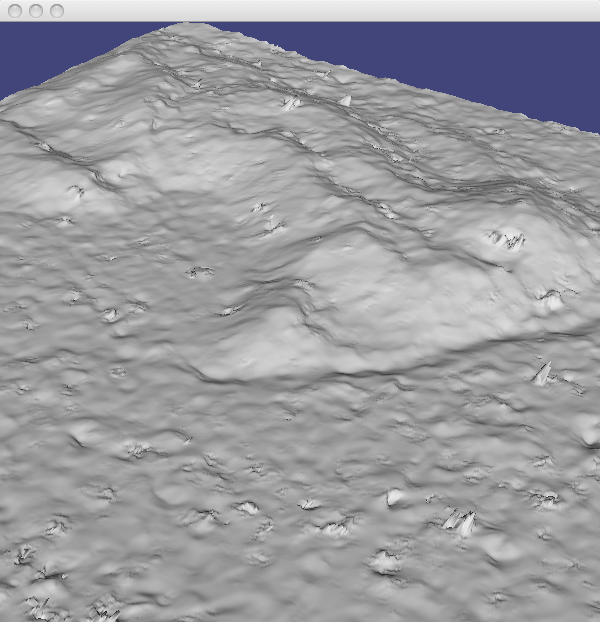
\includegraphics[width=3in]{images/correlation/3D_mode2.png}}
  \hfil
  \subfigure[{\tt Hillshade Result}]{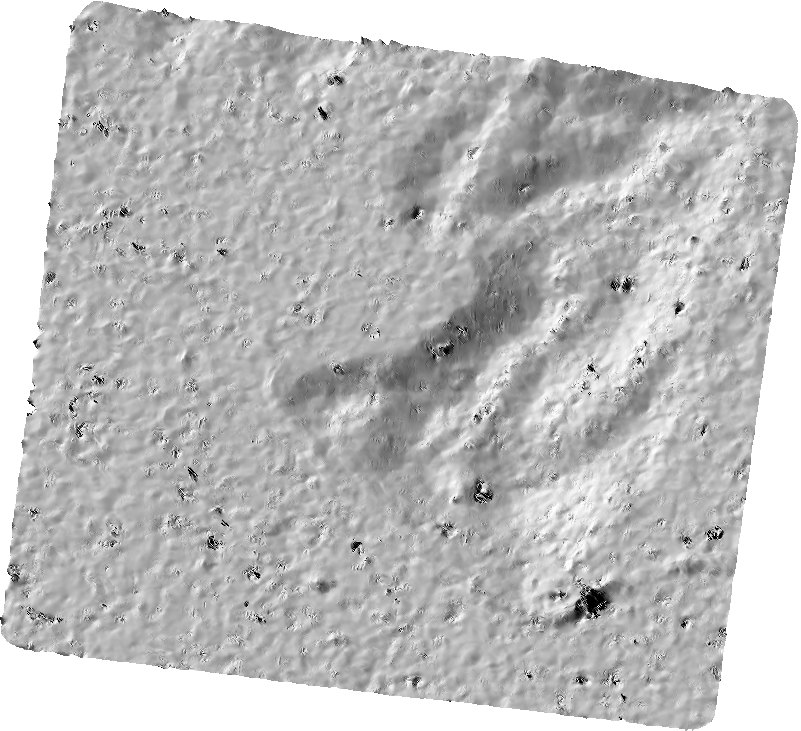
\includegraphics[width=3in]{images/correlation/hillshade_mode2.png}}
\caption{Results using Bayes weighted Affine subpixel mode.}
\label{fig:bayes_results}
\end{figure}

\subsection{Bayes EM weighted Affine}

\begin{figure}[hb]
\centering
  \subfigure[{\tt 3D result}]{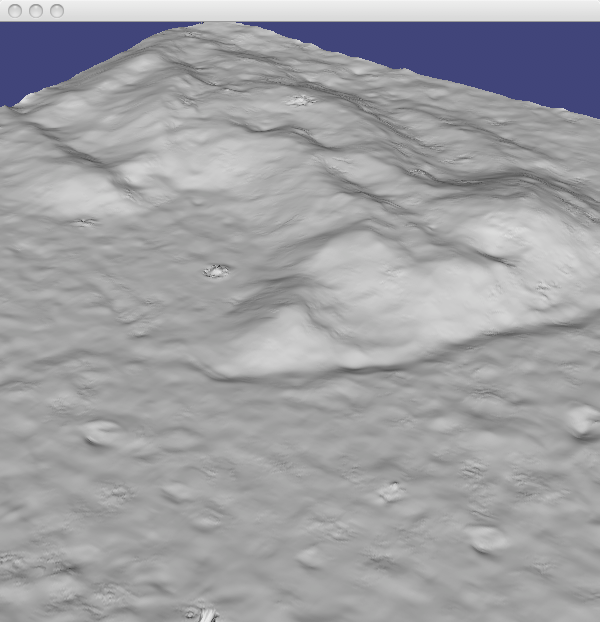
\includegraphics[width=3in]{images/correlation/3D_mode3.png}}
  \hfil
  \subfigure[{\tt Hillshade Result}]{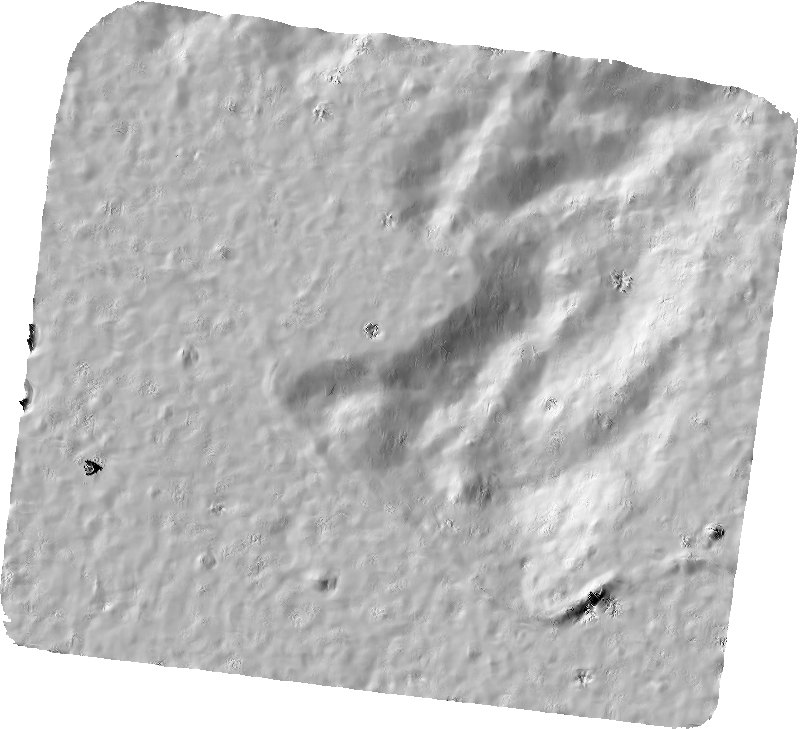
\includegraphics[width=3in]{images/correlation/hillshade_mode3.png}}
\caption{Results using Bayes EM weighted Affine subpixel mode.}
\label{fig:bayes_em_results}
\end{figure}
